\newpage
\section{Modelli linari}
\subsection{Regression}
Un possibile esempio di regressione potrebbe essere un processo di stima di una funzione di valore
reale sulla base di un insieme finito di campioni rumorosi. Le conoscenze sarebbero $pairs(x, f(x) + random noise)$.\\
La task a questo punto sarebbe trovare $f$ per i dati nella seguente tabella.
\begin{figure}[h!]
    \centering
    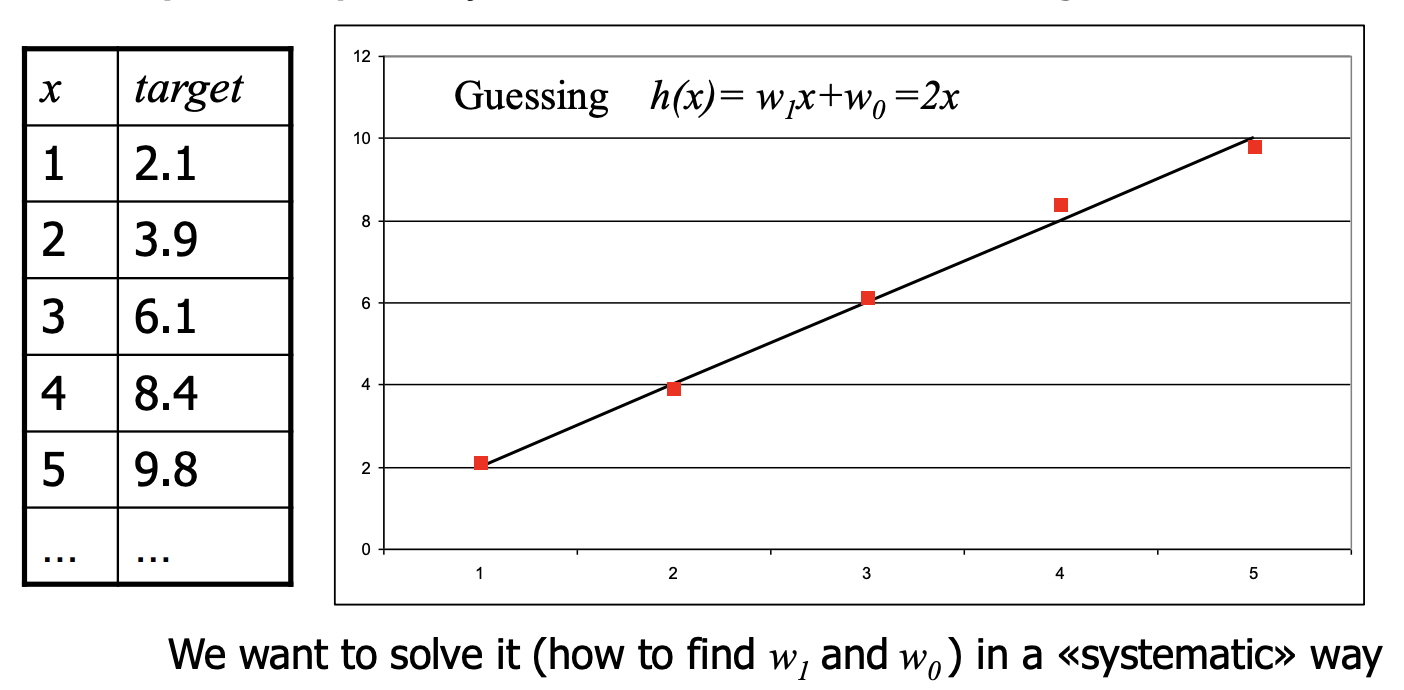
\includegraphics[width=0.65\textwidth]{images/esempio-regresione.png}
\end{figure}
\begin{example}
    Esempio di modelli linari:
    \begin{figure}[h!]
        \centering
        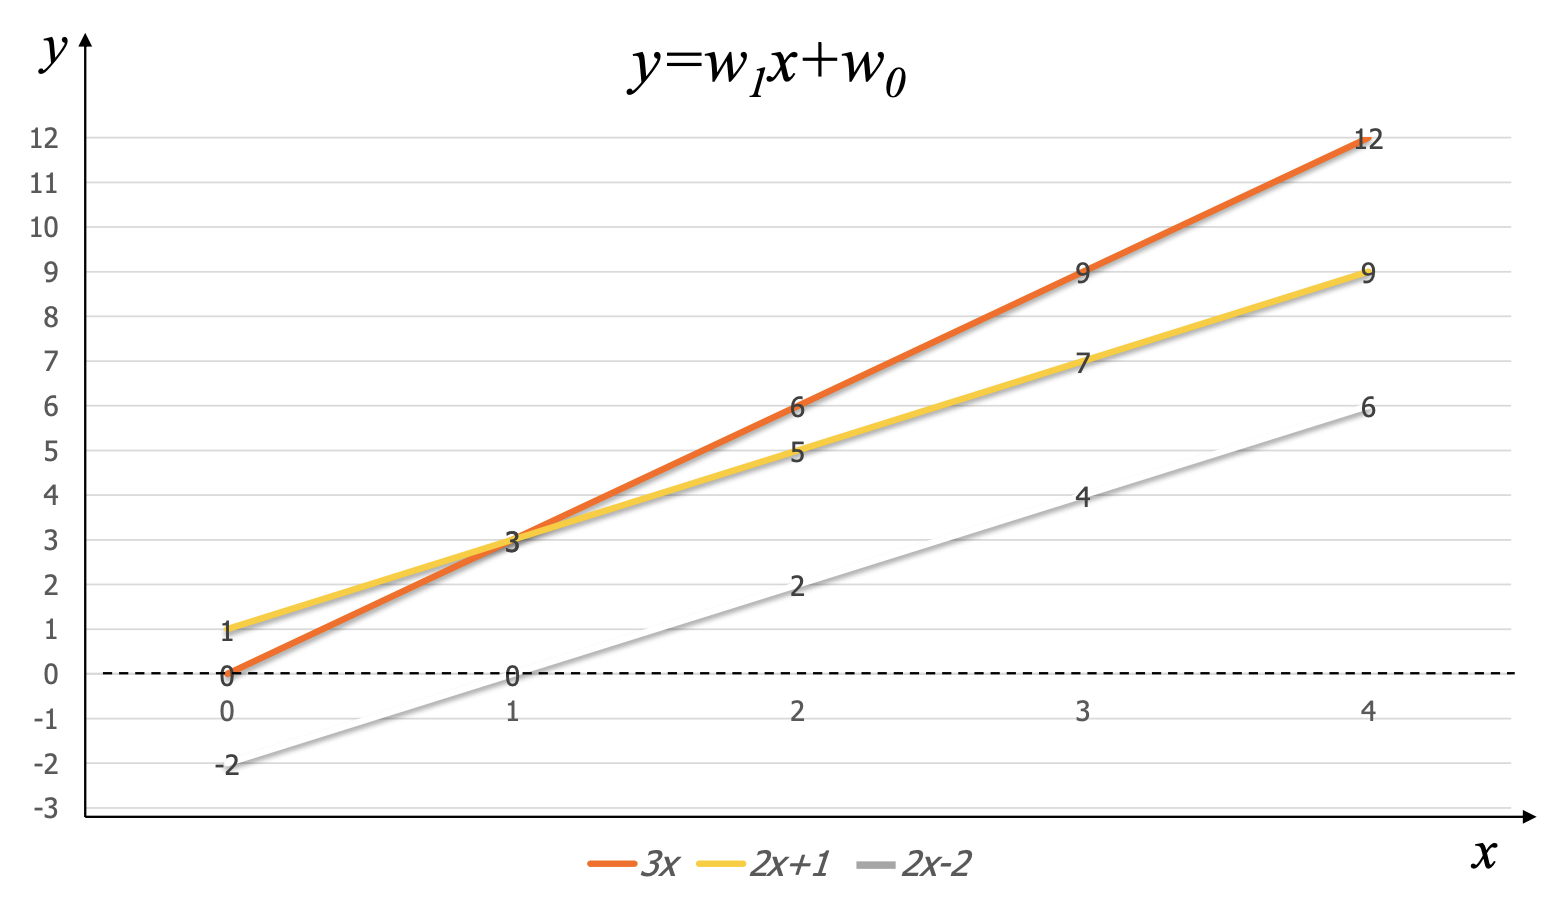
\includegraphics[width=0.65\textwidth]{images/esempio-modelli-lineari.png}
    \end{figure}
\end{example}

\subsubsection{Univariate linear regression}
Il caso univariante, semplice regressione linieare: iniziamo con 1 valore di inputl, $x$ e 
1 valore di output $y$.
\begin{definition}
    Assumiamo che un modello $h_w(x)$ espresso come:
    $$out = h(x) = w_1x + w_0$$
    dove $w$ è il coefficiente a valore reale/paramentro libero (peso).
\end{definition}
Si cerca di avere un adattamento dei dati secondo una “linea retta”. Trovare $h$ (modello lineare) che 
meglio si adattano ai dati (da gli insieme di dati osservati dei valori $x$ e $y$). Assumiamo che la variabile data (y) è (linearmente) 
associata ad un'altra viarialbe (x) o più variabili, da $y = w_1x + w_0 + noise$, dove $w$ è il free par e $noise$ è
un errore misurato al target (con una distribuzione normale). Andiamo a costruire un modello (trovare il valore $w$) per predirre/stimare il prezzo ($y$) dei punti
per altri (osservabile) valori $x$ (prediction).
\begin{figure}[h!]
    \centering
    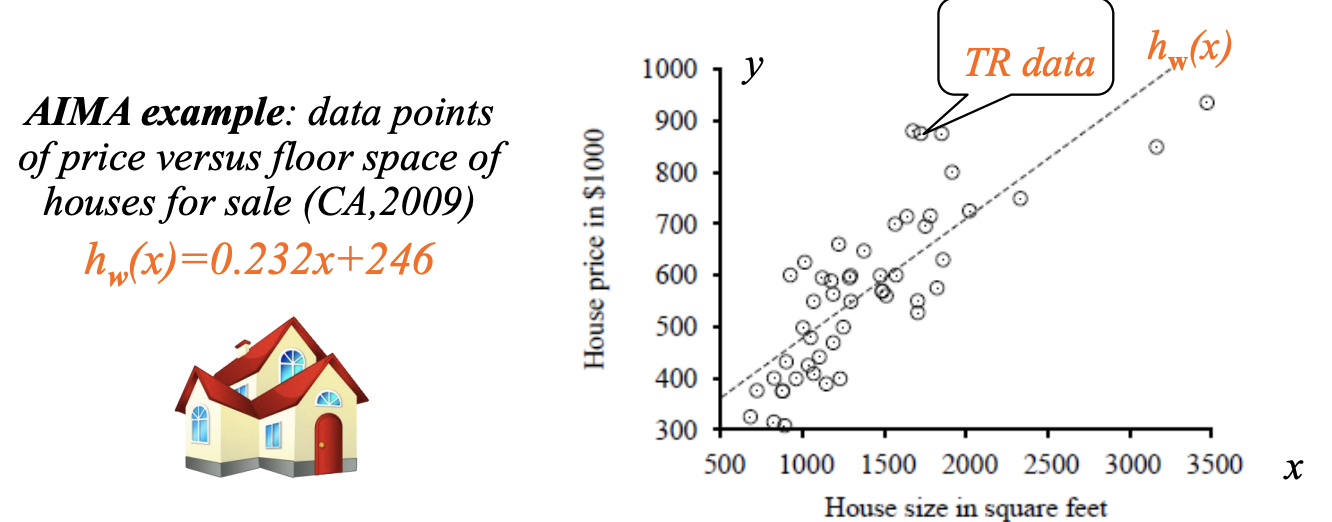
\includegraphics[width=0.6\textwidth]{images/task-model-esempio.png}
\end{figure}
Usiamo poi questi valori per \textbf{predirre/stimare} il prezzo (t) dei punti per altri valore osservabili.
\begin{figure}[h!]
    \centering
    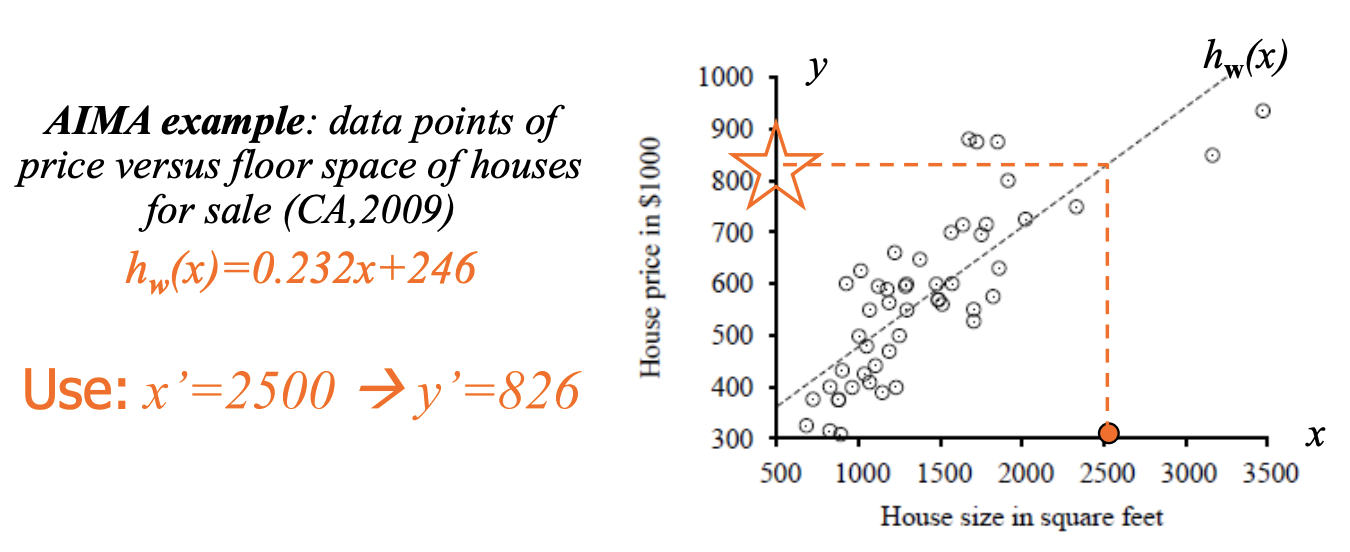
\includegraphics[width=0.6\textwidth]{images/uso-predizione-esempio.png}
\end{figure}

\subsubsection{Learning via LMS}
Abbiamo capito che quindi dobbiamo andare a trovare i valori dei paramentri $w$ ($w_1$ e $w_2$ nei casi univarianti) per andare a minimizzare 
l'output dell'errore del modello (per eseguire un buon fitting). In uno spazio di ipotesi infinito (valore $w$ continuo) abbiamo una buona soluzione
data dalla matematica classica, possiamo "imparare" da dei semplici tools, sebbene semplice incluse moltri concetti rileventi per
il ML moderno ed è alla abse dei metodi evoluti in the field. Definiamo qui una \textbf{funzione less / error} e usiamo il \textbf{Least Mean Square (LMS)} approccio.\\\\
\textbf{Il training} si fa trovando $w$ tale che minimizzi l'\textbf{errore}/la \textbf{perdita epirica} (il miglior dato che fitta nel training set con l'esempio $l$)

\begin{definition}
    Andiamo allora a definire LMS con:
    \begin{itemize}
        \item \textbf{Given} un insieme ti esempi di training $l$ ($x_p, y_p$) $p = 1 \dots l$
        \item \textbf{Trovare} $h_w(x)$ nella forma $w_1 x + w_0$ (quindi i valori di $w$) che minimizzano la perdita attesa dei dati di training.
    \end{itemize}
    Per la perdita usiamo la radice dell'errore.\\
    Da qui il \textbf{least (mean) square} si tratta di trovare la $w$ che minimizzi la somma residua delle ragdici [$argmin_w Error(w) in L_2$]
    $$Loss(h_w) = E(w) = \sum_{p=1}^{l} (y_p - h_w(x_p))^2 = \sum_{p=1}^{l}(y_p - (w_1 x_p + w_0))^2$$
    Dove $x_p$ è $p-th$ input/pattern/esample, $y_p$ l'output per $p$, $w$ free par., $l$ numero degli esempi.
\end{definition}